\documentclass{article}
\usepackage[utf8]{inputenc}
\usepackage{graphicx}
\usepackage{amsmath}
\usepackage{float}


\title{
Clase 3: Ejercicio grupal - G10

Curso Nivelador Análisis – Carrera de Especialización en Estadística 2022
}

\author{Alejandro Uribe}
\date{Octubre 2022}

\begin{document}

\maketitle

\begin{enumerate}
    \item Dada $f(x) = \frac{1}{\sqrt{x^2-9}}$ con $x \in [-1, 2]$
    \begin{enumerate}
        \item Calcular $f'$, $Domf'$ y determinar los puntos críticos.
        \item Máximos y mínimos absolutos de $f$ en $[-1, 2]$.
    \end{enumerate}
    A fin de calcular $f'$, $Domf'$, puntos críticos de $f(x)$, y máximos y mínimos absolutos de $f(x)$, la función debe ser derivable en el intervalo $x\in[-1,2]$.
    
    El $Domf$, son aquellos valores de $x$ para los cuales existe un valor asociado de la función $f(x)$:
    $$Domf = \{ x \in \mathbf{R}\ / \quad \exists f(x)\}$$
    
    Se calcula el $Domf$:
    $$Domf = \{ x \in \mathbf{R}\ / \quad x^2-9 > 0\}$$
    Es decir,
    $$Domf = \{ x \in \mathbf{R}\ / \quad x<-3 \quad | \quad x>3 \}$$
    
    Por lo tanto, $f(x)$ no se encuentra definida en el intervalo $[-1,2]$ y no es derivable en tal intervalo.
    \item Dada $f(x) = \frac{1}{\sqrt{x^2-9}}$
    \begin{enumerate}
        \item Hallar el $Domf$
      
        El $Domf$ son aquellos valores de $x$ para los cuales existe un valor asociado de la función $f(x)$:
        $$Domf = \{ x \in \mathbf{R}\ / \quad \exists f(x)\}$$
      
        Se calcula el $Domf$:
        $$Domf = \{ x \in \mathbf{R}\ / \quad x^2-9 > 0\}$$
      
        Es decir,
        $$Domf = \{ x \in \mathbf{R}\ / \quad x<-3 \quad | \quad x>3 \}$$
      
        \item Para cada $c$ en el borde del dominio de $f(x)$, determinar qué límites laterales tiene sentido tomar cuando $x$ tiende a $c$ y calcularlos.
      
        El dominio de $f(x)$ es $Domf = (-\infty, -3) \cup (3, \infty)$. Por lo que tiene sentido tomar los límites cuando $x \to \{-3^-, 3^+, \pm \infty\}$. 
      
        $$\lim_{x\to \pm \infty} \frac{1}{\sqrt{x^2-9}} = 0$$
        $$\lim_{x\to -3^-} \frac{1}{\sqrt{x^2-9}} = +\infty$$
        $$\lim_{x\to 3^+} \frac{1}{\sqrt{x^2-9}} = +\infty$$
      
        \item Calcular $f'$, $Domf'$ y hallar sus puntos críticos. Luego analizar dónde crece y decrece $f$.
      
        \textbf{Calcular $f'$}
        $$\frac{d f(x)}{dx} = \frac{d}{d x} \left(\frac{1}{\sqrt{x^2-9}} \right)$$
        $$\frac{d f(x)}{dx}= -\frac{x}{(x^2-9)^{\frac{3}{2}}}$$
      
        \textbf{Calcular $Domf'$}
      
        El $Domf'$, son aquellos valores de $x$ para los cuales existe un valor asociado de la función $f'(x)$:
        $$Domf' = \{ x \in \mathbf{R}\ / \quad \exists f'(x)\}$$
        Se calcula el $Domf'$:
        $$Domf'= \{ x \in \mathbf{R}\ / \quad x^2-9 > 0\}$$
        Es decir,
        $$Domf'= \{ x \in \mathbf{R}\ / \quad x<-3 \quad | \quad x>3 \}$$
      
        \textbf{Puntos críticos}
      
        Los puntos críticos de $f(x)$ son los $x_i$ tales que $f'(x_i) = 0$.
        $$f'(x) = -\frac{x}{(x^2-9)^{\frac{3}{2}}}$$
        $$-\frac{x}{(x^2-9)^{\frac{3}{2}}} = 0$$
        $$\left(\frac{1}{(x^2-9)^{\frac{3}{2}}} \right) (-x) = 0$$
        Notar que $\left(\frac{1}{(x^2-9)^{\frac{3}{2}}} \right) > 0 \quad \forall x \in Domf'$. Por otro lado, $(-x)$ no toma el valor de cero ya que tal no pertence al $Domf'$. Por lo tanto, $f(x)$ no tiene puntos críticos en su dominio.
      
        \textbf{Intervalos $f(x)$ donde crece o decrece}
        \begin{itemize}
            \item $f(x)$ crece si $f'(x) > 0$, es decir:
            $$\left(\frac{1}{(x^2-9)^{\frac{3}{2}}} \right) (-x) > 0$$
            Notar que $\left(\frac{1}{(x^2-9)^{\frac{3}{2}}} \right) > 0 \quad \forall x \in Domf'$. Por otro lado, $(-x) > 0$ si $x < 0$.
            \item $f(x)$ decrece si $f'(x) < 0$, es decir:
            $$\left(\frac{1}{(x^2-9)^{\frac{3}{2}}} \right) (-x) < 0$$
            Notar que $\left(\frac{1}{(x^2-9)^{\frac{3}{2}}} \right) > 0 \quad \forall x \in Domf'$. Por otro lado, $(-x) > 0$ si $x > 0$.
        \end{itemize}
        Por lo tanto,
        \begin{equation*}
            \begin{cases}
                f'(x)> 0, & \text{si $x < -3 \Rightarrow f(x) \uparrow$}\\
                f'(x)< 0, & \text{si $x > 3 \Rightarrow f(x) \downarrow$}
            \end{cases}
        \end{equation*}
      
        \item Hallar máximos y mínimos locales y decidir si son absolutos.
      
        Del item anterior se concluyó que $f(x)$ no tiene puntos críticos. No obstante, $f(x)$ tiene dos asíntotas verticales: $x=-3, \quad x=3$ y una asíntota vertical en $y=0$.
      
        \item Esbozar un gráfico de $f$.
      
        De los items anteriores se tiene que:
        \begin{equation*}
            \text{Asíntotas}\begin{cases}
                \text{Horizontales}: & \left\{ \text{$y=0$} \right\}\\
                \text{Verticales}: & \left\{ \text{$x=-3, \quad x=3$} \right\}
            \end{cases}
        \end{equation*}
        
        \begin{equation*}
            \text{Crecimiento/Decrecimiento}\begin{cases}
            \text{$f(x) \uparrow$}, & \text{si $x<-3$} \\ 
            \text{$f(x) \downarrow$}, & \text{si $x>3$}
            \end{cases}
        \end{equation*}
        
        Resta analizar la concavidad de $f(x) \quad \forall x \in Domf$. Para ello se calcula la segunda derivada de $f(x)$.
        
        $$\frac{d^2f(x)}{dx^2} = \frac{d^2}{dx^2} \left(\frac{1}{\sqrt{x^2-9}} \right)$$
        $$\frac{d^2f(x)}{dx^2} = \frac{2x^2 - 9}{(x^2 -9)^{\frac{5}{2}}}$$
        
        La función $f(x)$ es cóncava hacia abajo si $f"(x) < 0$ y cóncava hacia arriba si $f"(x) > 0$. Al tomar valores arbitarios de $x \in Domf$, se nota que:
        
        \begin{equation*}
            \begin{cases}
                \text{$f"(x)>0$}, & \text{si \{$x<-3, \quad x>3\}$} \\
                \text{$f"(x) < 0$}, & \text{en ningún caso}
            \end{cases}
        \end{equation*}
        
        Se esboza la gráfica de $f(x)$ a continuación.
      
        \begin{figure}[H]
            \centering
            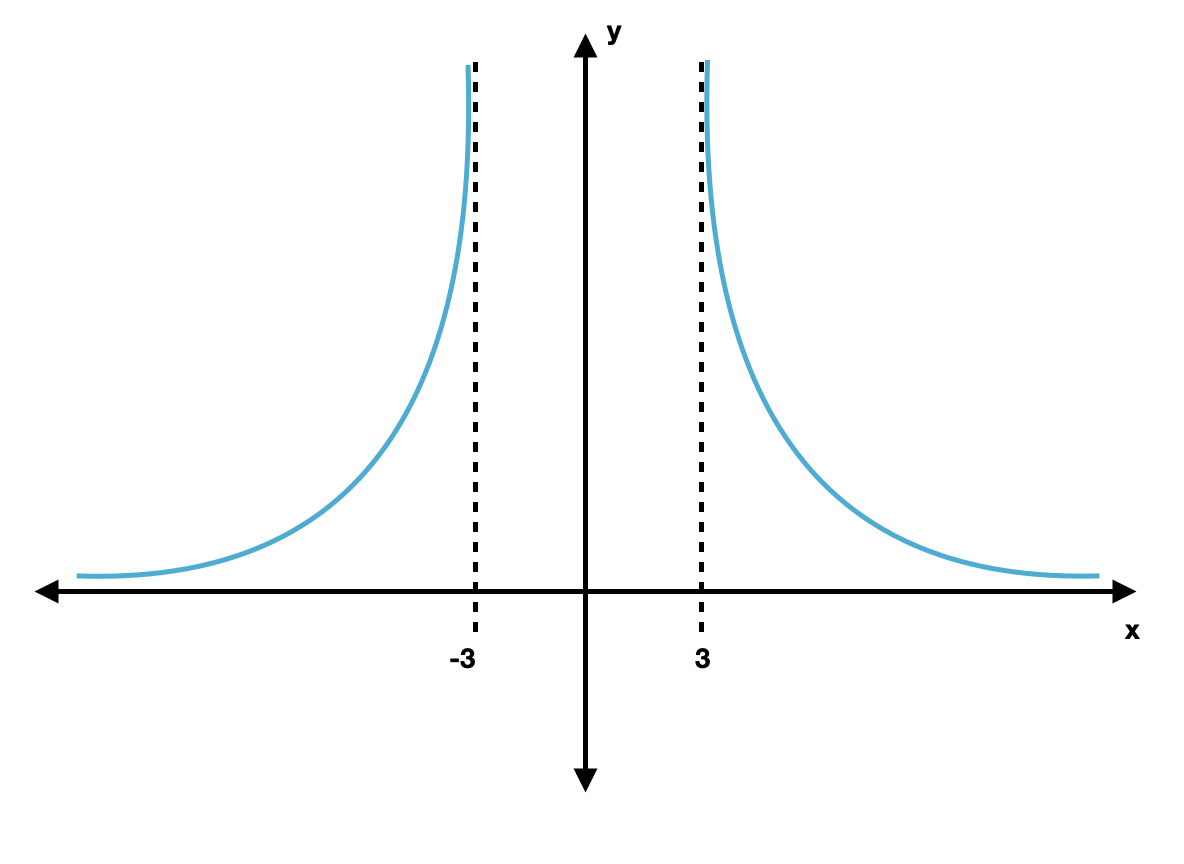
\includegraphics[width=9cm]{ChartIO}
        \end{figure}

        \item Hacer un gráfico de la función usando la computadora y comparar con el gráfico del item anterior.
            \begin{figure}[H]
                \centering
                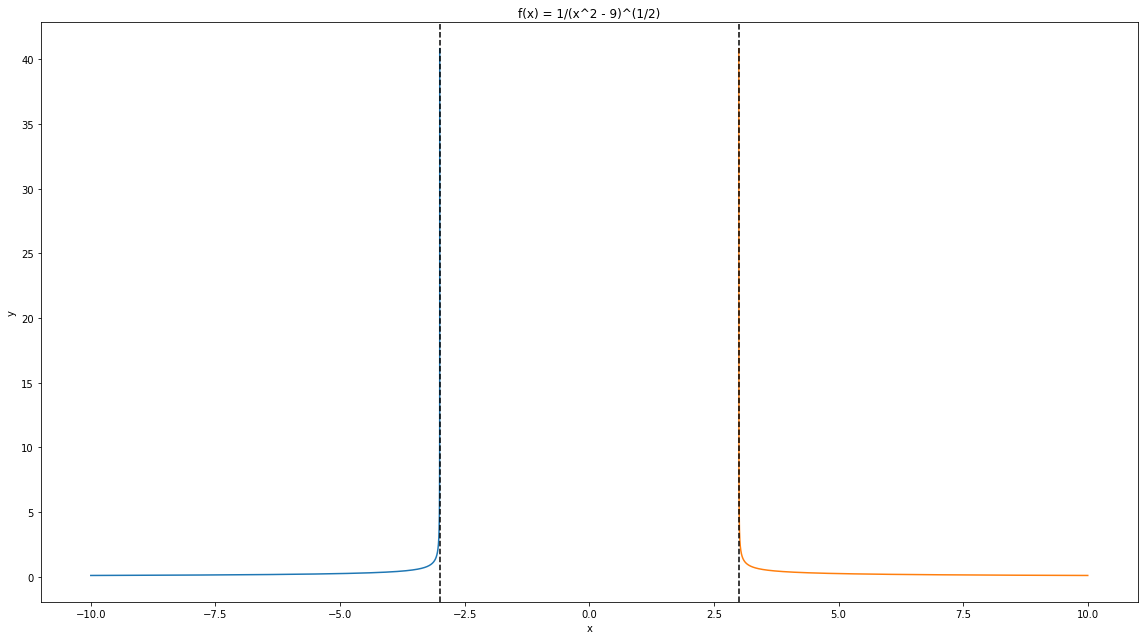
\includegraphics[width=9cm]{image.png}
            \end{figure}
            
        Notar que la función generada por computadora se acerca mas rápido a sus asíntotas verticales y horizontales que en el esbozo a mano.
        
      \item Decidir si son verdaderas o falsas cada una de las siguientes afirmaciones
      \begin{enumerate}
        \item $f(x) \leq 1/3 \quad \forall x \in Domf$
            Se chequea tal condición:
            $$\frac{1}{\sqrt{x^2-9}} \leq \frac{1}{3}$$
            La condición se cumple si:
            $$x \geq 3\sqrt{2}$$
            Y se sabe que:
            $$Domf = \{ x \in \mathbf{R}\ / \quad x<-3 \quad | \quad x>3 \}$$
            Por lo tanto, la afirmación es falsa.
          \item $f(x) < 1/2 \quad \forall x \in Domf$
            Se chequea tal condición:
            $$\frac{1}{\sqrt{x^2-9}} \leq \frac{1}{2}$$
            La condición se cumple si:
            $$x \geq \sqrt{13}$$
            Y se sabe que:
            $$Domf = \{ x \in \mathbf{R}\ / \quad x<-3 \quad | \quad x>3 \}$$
            Por lo tanto, la afirmación es falsa.
      \end{enumerate}
  \end{enumerate}
\end{enumerate}

\end{document}
